%%%%%%%%%%%%%%%%%%%%%%%%%%%%%%%%%%%%%%%%%
% Wenneker Assignment
% LaTeX Template
% Version 2.0 (12/1/2019)
%
% This template originates from:
% http://www.LaTeXTemplates.com
%
% Authors:
% Vel (vel@LaTeXTemplates.com)
% Frits Wenneker
%
% License:
% CC BY-NC-SA 3.0 (http://creativecommons.org/licenses/by-nc-sa/3.0/)
% 
%%%%%%%%%%%%%%%%%%%%%%%%%%%%%%%%%%%%%%%%%

%----------------------------------------------------------------------------------------
%	PACKAGES AND OTHER DOCUMENT CONFIGURATIONS
%----------------------------------------------------------------------------------------

\documentclass[11pt]{article} % Font size

%%%%%%%%%%%%%%%%%%%%%%%%%%%%%%%%%%%%%%%%%
% Wenneker Assignment
% Structure Specification File
% Version 2.0 (12/1/2019)
%
% This template originates from:
% http://www.LaTeXTemplates.com
%
% Authors:
% Vel (vel@LaTeXTemplates.com)
% Frits Wenneker
%
% License:
% CC BY-NC-SA 3.0 (http://creativecommons.org/licenses/by-nc-sa/3.0/)
% 
%%%%%%%%%%%%%%%%%%%%%%%%%%%%%%%%%%%%%%%%%

%----------------------------------------------------------------------------------------
%	PACKAGES AND OTHER DOCUMENT CONFIGURATIONS
%----------------------------------------------------------------------------------------

\usepackage{amsmath, amsfonts, amsthm} % Math packages

\usepackage{float}

\usepackage{color}

\usepackage{listings} % Code listings, with syntax highlighting

\usepackage[english]{babel} % English language hyphenation

\usepackage{graphicx} % Required for inserting images
\graphicspath{{Figures/}{./}} % Specifies where to look for included images (trailing slash required)

\usepackage{booktabs} % Required for better horizontal rules in tables

\numberwithin{equation}{section} % Number equations within sections (i.e. 1.1, 1.2, 2.1, 2.2 instead of 1, 2, 3, 4)
\numberwithin{figure}{section} % Number figures within sections (i.e. 1.1, 1.2, 2.1, 2.2 instead of 1, 2, 3, 4)
\numberwithin{table}{section} % Number tables within sections (i.e. 1.1, 1.2, 2.1, 2.2 instead of 1, 2, 3, 4)

\setlength\parindent{0pt} % Removes all indentation from paragraphs

\usepackage{enumitem} % Required for list customisation
\setlist{noitemsep} % No spacing between list items

%----------------------------------------------------------------------------------------
%	DOCUMENT MARGINS
%----------------------------------------------------------------------------------------

\usepackage{geometry} % Required for adjusting page dimensions and margins

\geometry{
	paper=a4paper, % Paper size, change to letterpaper for US letter size
	top=2.5cm, % Top margin
	bottom=3cm, % Bottom margin
	left=3cm, % Left margin
	right=3cm, % Right margin
	headheight=0.75cm, % Header height
	footskip=1.5cm, % Space from the bottom margin to the baseline of the footer
	headsep=0.75cm, % Space from the top margin to the baseline of the header
	%showframe, % Uncomment to show how the type block is set on the page
}

%----------------------------------------------------------------------------------------
%	FONTS
%----------------------------------------------------------------------------------------

\usepackage[utf8]{inputenc} % Required for inputting international characters
\usepackage[T1]{fontenc} % Use 8-bit encoding

\usepackage{fourier} % Use the Adobe Utopia font for the document

%----------------------------------------------------------------------------------------
%	SECTION TITLES
%----------------------------------------------------------------------------------------

\usepackage{sectsty} % Allows customising section commands

\sectionfont{\vspace{6pt}\centering\normalfont\scshape} % \section{} styling
\subsectionfont{\normalfont\bfseries} % \subsection{} styling
\subsubsectionfont{\normalfont\itshape} % \subsubsection{} styling
\paragraphfont{\normalfont\scshape} % \paragraph{} styling

%----------------------------------------------------------------------------------------
%	HEADERS AND FOOTERS
%----------------------------------------------------------------------------------------

\usepackage{scrlayer-scrpage} % Required for customising headers and footers

\ohead*{} % Right header
\ihead*{} % Left header
\chead*{} % Centre header

\ofoot*{} % Right footer
\ifoot*{} % Left footer
\cfoot*{\pagemark} % Centre footer
 % Include the file specifying the document structure and custom commands

\title{	
	\normalfont\normalsize
	
\includegraphics[width=0.5\columnwidth]{logo-black}
	%\textsc{Molo17 S.r.l.}\\ % Your university, school and/or department name(s)
	\vspace{25pt} % Whitespace
	\rule{\linewidth}{0.5pt}\\ % Thin top horizontal rule
	\vspace{20pt} % Whitespace
	{\huge Event-Driven cloud architectures, CQRS and Event Sourcing}\\ % The assignment title
	\vspace{12pt} % Whitespace
	\rule{\linewidth}{2pt}\\ % Thick bottom horizontal rule
	\vspace{12pt} % Whitespace
}

\author{\LARGE Lorenzo Busin} % Your name

\date{\normalsize August, 2019} % Today's date (\today) or a custom date

\begin{document}

\maketitle % Print the title

%\section{Image Interpretation}

%\begin{figure}[h] % [h] forces the figure to be output where it is defined in the code (it suppresses floating)
	%\centering
	%\includegraphics[width=0.5\columnwidth]{swallow.jpg} % Example image
	%\caption{European swallow.}
%\end{figure}
\tableofcontents
\newpage

\section{Event-Driven architectures}  

\subsection{What is an Event-Driven architecture?}
Event-Driven architecture is a popular distributed asynchronous architecture pattern used to produce highly scalable and adaptable applications. It is made of highly decoupled and single-purpose event processing components that receive and process events. 

\subsection{What is an event?}
An event is an action recognized and handled by the software, often asynchronously. Events can be generated or triggered by the system, the user or in other ways. The software can also trigger its own set of events to forward information to other services or communicate with them. An application that changes its behavior in response to events is called "Event-Driven".\\
The main difference between commands and events is that the firsts say to the system \emph"This is what you have to do" while the seconds just say \emph{"This is happened"} and then is up the handler to decide what to do.

\subsection{What is Event-Driven programming?}
Event-Driven programming is a programming paradigm where the flow of the program is determined by events such as user actions, sensor outputs or messages from other programs. This paradigm is mostly used in graphical user interfaces and other applications such as JavaScript web apps that are centered on performing actions in response to inputs. \\
In an Event-Driven application there is a main loop that listens for events and then triggers a callback function when one of those is detected. The events listener is a common thing among applications, for this reason many programming frameworks take care of their implementation and expect the user to provide only the code for the event handlers.

\subsection{Events communication}
Events just communicate that something happened, so with them you let a system know that something has happened. When an event occurs it will activate its handler which implements the execution logic. The result of the event's execution can turn into changes in the model-view or can trigger other handlers by forwarding it. \\
The \emph{observer} pattern is a flawless example of how events communicate with each other. 
\begin{figure} [H]
	\centering
	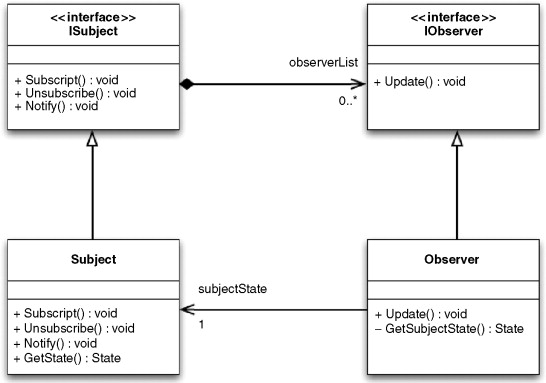
\includegraphics[scale=0.8]{observer}
\end{figure}
A subject maintains a list of its  observers and notifies them automatically of any state changes, usually by calling one of their methods.
This design pattern is mainly used to implement distributed event handling systems and is also a key part in MVC pattern.\\ 

According to \emph{Martin Fowler}, there are two ways of communicating between events: \textbf{Event notification} and \textbf{Event-Carried State Transfer}.

\subsubsection{Event notification}
To understand how Event notification works we can think of when our smartphone notifies us that a new message has arrived without adding any information. This happens when a system sends event messages to notify other systems of a change in its domain. The receiver knows something has changed but then issues a request back to the sender to decide what to do next, sending a request message and receiving a response for every event that happened. \\
The key element of Event notification is that the source system doesn't really care much about the response. So if the event's body does not need, Event notification is an excellent solution as it guarantees decoupling and high performance.

\subsubsection{Event-Carried State Transfer}
To understand how Event-Carried State Transfer works we can think of when our smartphone notifies us that a new message has arrived but in this case it shows other information like the sender's name and the message content. When an something changes, the event that is generated contains the details of what has been changed. In this way the receiver does not need to ask the sender what has been changed.\\
A down-side of this model is that the messages that are sent contain more data but this reduce latency, because it is not necessary to query the source for further details. It does involve more complexity on the receiver since it has to sort out maintaining all the state, when it's usually easier just to call the sender to obtain more information.\\
So if the receiver needs to know extra data with the event object, Event-Carried State Transfer is an excellent solution as it guarantees better performance and lower demands on the supplier, but more expensive communications.


\subsection{Event-Driven architecture's topologies}
Event-Driven architecture consists of two main topologies: \textbf{mediator} and \textbf{broker}. The mediator one is commonly used when you need to orchestrate multiple steps within an event through a central mediator, whereas the broker topology is used when you want to chain events together without the use of a central mediator.

\subsubsection{Mediator topology}
The mediator topology is useful for events that have multiple steps and require some level of orchestration to process the event. For example, a single event may consist of multiple steps that would require a certain level of orchestration to determine their order of execution \\
There are four main types of architecture components within the mediator topology: event \emph{queues}, an event \emph{mediator}, event \emph{channels} and event \emph{processors}. \\
The event flow starts with a client sending an event to an event queue, which is used to transport the event to the mediator. It receives the initial event and orchestrates that event by sending additional events to event channels. Then, the event processors listen on the channels, receive the event and execute specific business logic.

\begin{figure} [H]
	\centering
	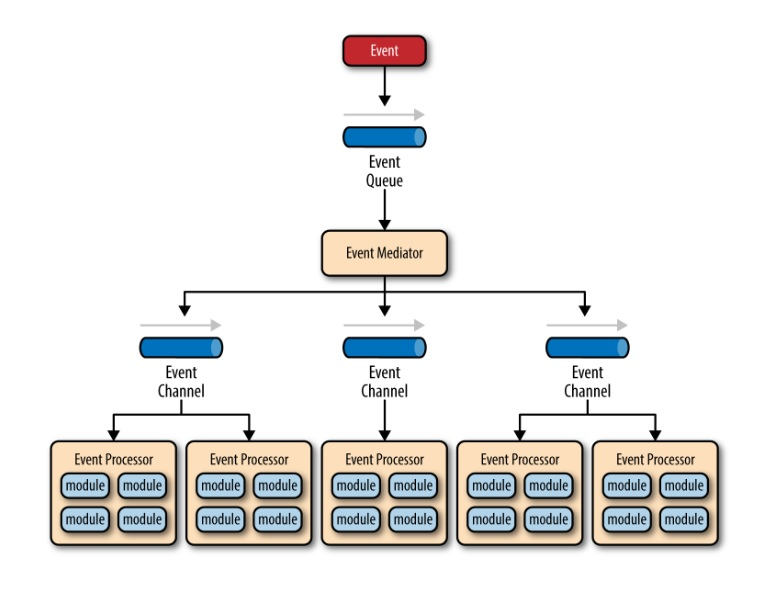
\includegraphics[scale=0.8]{mediator}
\end{figure}
There are two types of events within this pattern: an initial event and a processing event. The initial event is the original event received by the mediator, whereas the processing events are ones that are generated by the mediator and received by the event-processing components.\\
The event-mediator component is responsible for orchestrating the steps contained within the initial event. For each step in the initial event, the event mediator sends out a specific processing event to an event channel, which is then received and processed by the event processor. It is important to note that the event mediator doesn't actually perform the business logic necessary to process the initial event; rather, it knows of the steps required to process the initial event.\\
Event channels are used by the event mediator to asynchronously pass specific processing events related to each step in the initial event to the event processors. The event channels can be either message queues or message topics, although message topics are most widely used with the mediator topology so that processing events can be processed by multiple event processors (each performing a different task based on the processing event received).\\
The event processor components contain the application business logic necessary to process the processing event. Event processors are self-contained, independent, highly decoupled architecture components that perform a specific task in the application or system. While the granularity of the event-processor component can vary from fine-grained (e.g. calculate sales tax on an order) to coarse-grained (e.g. process an insurance claim), it is important to keep in mind that in general, each event-processor component should perform a single business task and not rely on other event processors to complete its specific task.

\subsubsection{Broker topology}
The broker topology differs from the mediator topology in that there is no central event mediator; rather, the message flow is distributed across the event processor components in a chain-like fashion through a lightweight message broker. This topology is useful when you have a relatively simple event processing flow.

\begin{figure} [H]
	\centering
	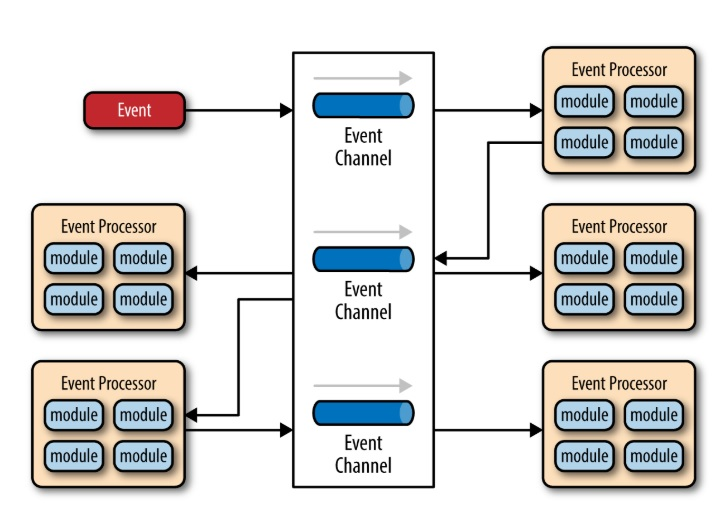
\includegraphics[scale=0.8]{broker}
\end{figure}

As you can see from the diagram, there is no central event-mediator component controlling and orchestrating the initial event; rather, each event-processor component is responsible for processing an event and publishing a new event indicating the action it just performed. For example, an event processor that balances a portfolio of stocks may receive an initial event called stock split. Based on that initial event, the event processor may do some portfolio rebalancing, and then publish a new event to the broker called rebalance portfolio, which would then be picked up by a different event processor. 

\subsubsection{Hybrid topology}
You can integrate both topologies, specially when you have to build a complex system.

\subsection{Pattern analysis}
\begin{figure} [H]
	\centering
	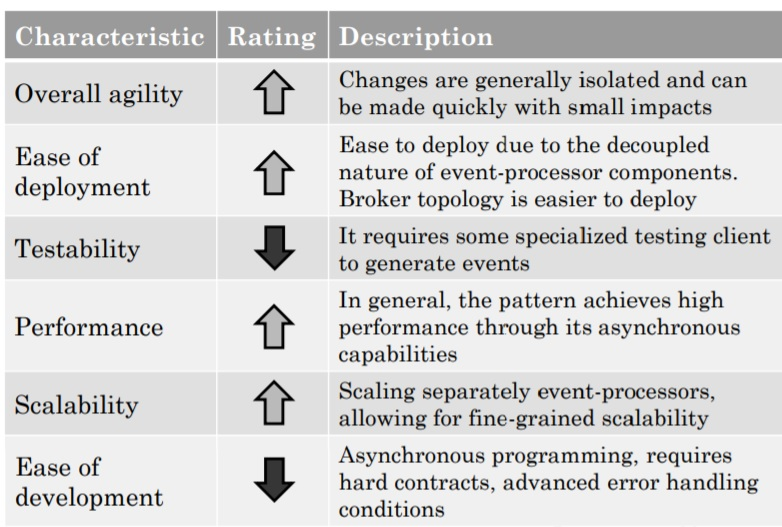
\includegraphics[scale=0.8]{analysis}
\end{figure}
\definecolor{darkgreen}{rgb}{0.0, 0.5, 0.0}
 \textbf{Overall agility}(\color{darkgreen}High\color{black}): is the ability to respond quickly to a constantly changing environment. Since event-processor components are single-purpose and completely decoupled from other event processor components, changes are generally isolated to one or a few event processors and can be made quickly without impacting other components; \\
 \textbf{Ease of deployment}(\color{darkgreen}High\color{black}): this pattern is relatively easy to deploy due to the decoupled nature of the event-processor components. The broker topology tends to be easier to deploy than the mediator topology, primarily because the event mediator component is somewhat tightly coupled to the event processors: a change in an event processor component might also require a change in the event mediator, requiring both to be deployed for any given change; \\
 \textbf{Testability}(\color{red}Low\color{black}): while individual unit testing is not overly difficult, it does require some sort of specialized testing client or testing tool to generate events. Testing is also complicated by the asynchronous nature of this pattern; \\
 \textbf{Performance}(\color{darkgreen}High\color{black}): the pattern achieves high performance through its asynchronous capabilities; \\
 \textbf{Scalability}(\color{darkgreen}High\color{black}): is naturally achieved in this pattern through highly independent and decoupled event processors; \\
 \textbf{Ease of development}(\color{red}Low\color{black}): development can be somewhat complicated due to the asynchronous nature of the pattern as well as contract creation and the need for more advanced error handling.

\newpage
\section{CQRS} 
\subsection{What is CQRS?}
\textbf{Command Query Responsibility Segregation} is an architectural pattern which separates the responsibility for modifying data(\emph{Command}) from reading them(\emph{Query}). The change that CQRS introduces is to split the conceptual model into separate models for updating and displaying data. The use of distinct models for writing and reading allows the infrastructure to easily scale to best fit the needs and allows to design and optimize each model for its responsibilities; this also allows the selection of the most appropriate technologies.

\subsection{When using CQRS?}
CQRS fits well with CRUD operations and with event-based programming models.
The adoption of this design pattern is strongly recommended in complex domains, where a single model to handle both reads and writes gets too hard but it can be made easier by separating the two models. Also, often happens that the number of writes in a system is lower than the number of readings so this pattern guarantees high performance avoiding traffic slowdown.

\subsection{How to implement CQRS?}
In complex applications usually happens that different services are integrated and the event's workflow from its birth until its complete execution often goes through different phases(calling different functions, different tasks etc.) while a reading operation just have to query a database to retrieves the needed data. \\
In these cases the ideal solution is to separate the system into two independent models: one for writing operations, which perform changes to the database and one for reading operations, which do not change anything.
  
\begin{figure} [H]
  \centering
  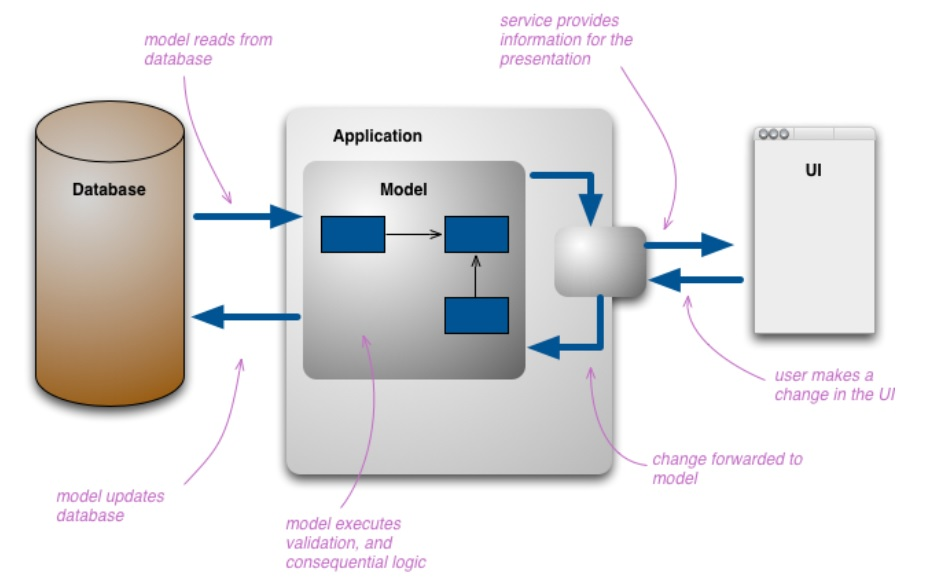
\includegraphics[scale=0.8]{CQRS1} \\
  Example of application model that \textbf{not} adopts CQRS
\end{figure}
\begin{figure} [H]
  \centering
  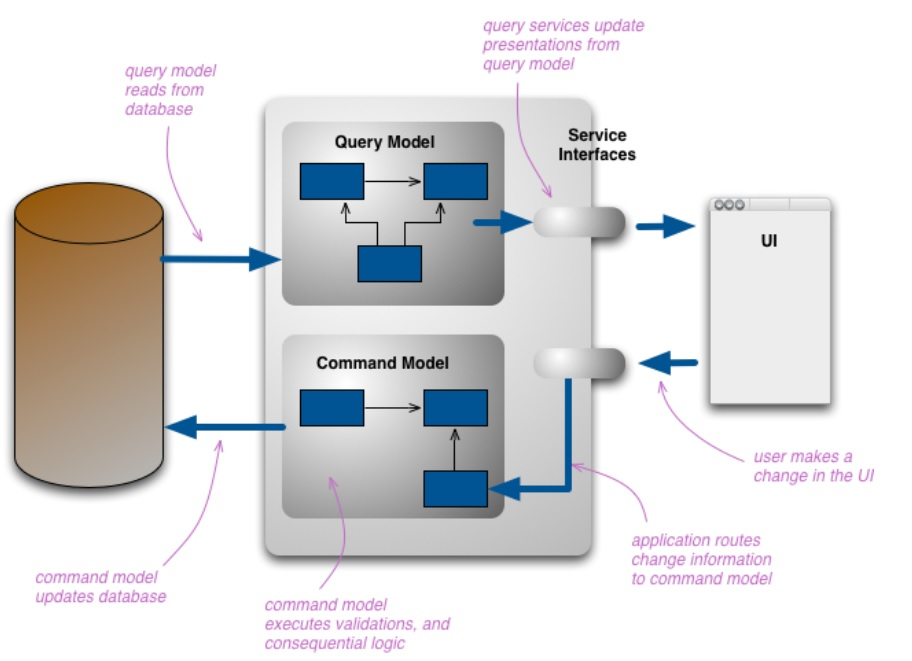
\includegraphics[scale=0.8]{CQRS2} \\
  Example of application model that adopts CQRS \\
\end{figure} 
\newpage
\section{Event Sourcing} 

\newpage
\section{Comparison between cloud providers} 

\end{document}
